\section{The Models}
\label{sec:models}

Due to the real-time nature of this application, we are using
a recursive Bayesian filtering approach as is often used in
real-time tracking applications.
We are using two distinct models for the vehicle and network states,
and in each assume an underlying Markov process with state $\mathcal{X}_k$
with system noise $\omega_k\sim\mathrm{N}(0,\mathcal{Q})$ 
of which observations $\mathcal{Y}_k$ are made
with error $\nu_k\sim\mathrm{N}(0,\mathcal{R})$,
giving the following general model below.
\begin{equation}
\label{eq:rbe_model}
\begin{split}
\mathcal{X}_k &= f(\mathcal{X}_{k-1}, \omega_k) \\
\mathcal{Y}_k &= h(\mathcal{X}_k, \nu_k)
\end{split}
\end{equation}
The transition function $f$ determines the relationship between consecutive states,
while the measurement function $h$ is a deterministic function describing the
relationship between the underlying and observed states.

The following sections describe the two models used in this application.
The first is implemented using a particle filter to estimate vehicle states,
with the primary objective of infering vehicle travel times along roads
from a sequence of GPS positions,
while the second uses these travel times to update road states 
and is implemented using an \emph{information filter},
which is a variant of the Kalman filter \citep{}.

\subsection{Real-time vehicle model}
\label{sec:pf}

The underlying vehicle state at time $t_k$ consists of
the vehicle's distance traveled $x$ in meters along the route and
it's speed $\dot x$ in meters per second.
Additionally, travel times along road segments along the route, 
$\bz = (z_1,\ldots,z_L)^\top$, in seconds,
are independent of time but included in the state so they can be estimated
sequentially as the vehicle traverses the route.
These are combined into the state vector,
\begin{equation}
\label{eq:vehicle_state}
\bX_k = 
\begin{bmatrix}
    x_k \\ \dot x_k \\ \bz
\end{bmatrix}.
\end{equation}
Observations $\bY_k$ of the vehicle are made using a GPS at time $t_k$
with GPS error $\epsilon^2$,
giving the longitude $\lambda_k$ and latitude $\phi_k$ of the vehicle,
\begin{equation}
\label{eq:vehicle_obs}
\bY_k = \begin{bmatrix} \lambda_k \\ \phi_k \end{bmatrix}.
\end{equation}


We chose to employ a particle filter to estimate $\bX_k$,
due to do its high flexibility and use in recent 
transit vehicle modeling applications \citep{Hans_2015}.
The primary advante of a particle filter is its handling of multimodality,
as in figure~\ref{fig:pf_state_predict},
which is a common feature of the proposal distribution, particularly around bus stops.
A second advantage is the intuitive likelihood function (see section~\ref{sec:pf_update}).
Conversely, particle filter methods are computationally demanding,
requiring an increasing number of particles as the model complexity and
number of parameters in increase \citep{}.
Section~\ref{sec:rt} describes our implementation of the particle filter in real-time 
and it's timings.



\begin{figure}[tb]
    \centering
    \begin{subfigure}[t]{0.48\textwidth}
        \centering
        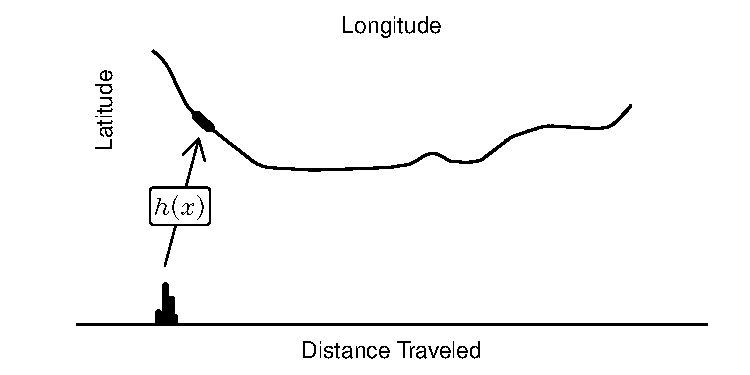
\includegraphics[width=\textwidth]{figures/03_particle_filter_1.pdf}
        \caption{The vehicle state represented by a sample of discrete points is related to the observable state (GPS position) through the transition function $h$.}
        \label{fig:pf_state_prev}
    \end{subfigure}\;\;
    \begin{subfigure}[t]{0.48\textwidth}
        \centering
        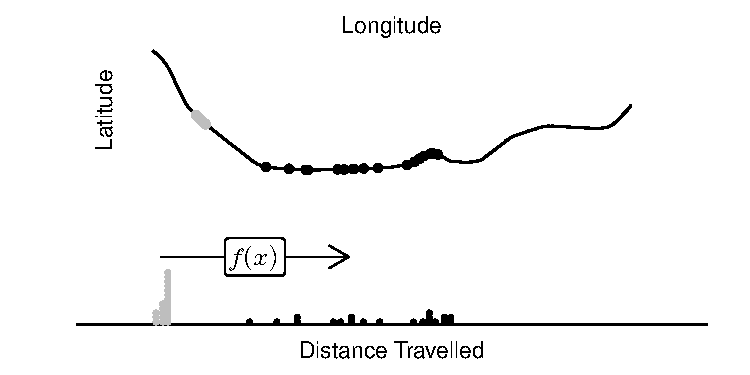
\includegraphics[width=\textwidth]{figures/03_particle_filter_2.pdf}
        \caption{The transition function $f$ models the behaviour of each particle,
            including changes in acceleration and stopping behaviour at bus stops.}
        \label{fig:pf_state_predict}
    \end{subfigure}\\
    \begin{subfigure}[t]{0.48\textwidth}
        \centering
        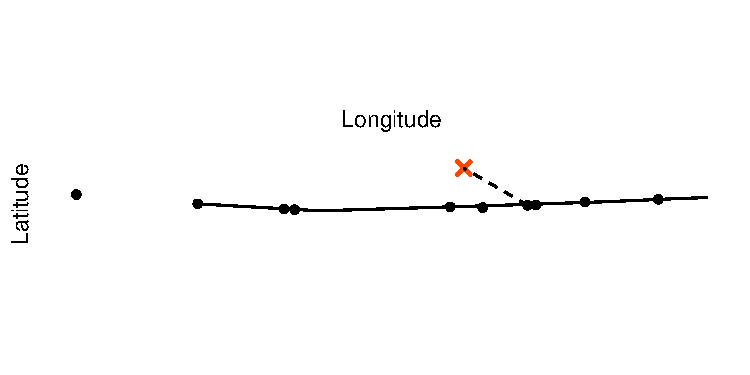
\includegraphics[width=\textwidth]{figures/03_particle_filter_6.pdf}
        \caption{Each particle's distance from the true observation is calculated using
            the geographic distance between two coordinates, which can then be used
            to calculate it's weight.}
        \label{fig:pf_state_update}
    \end{subfigure}\;\;
    \begin{subfigure}[t]{0.48\textwidth}
        \centering
        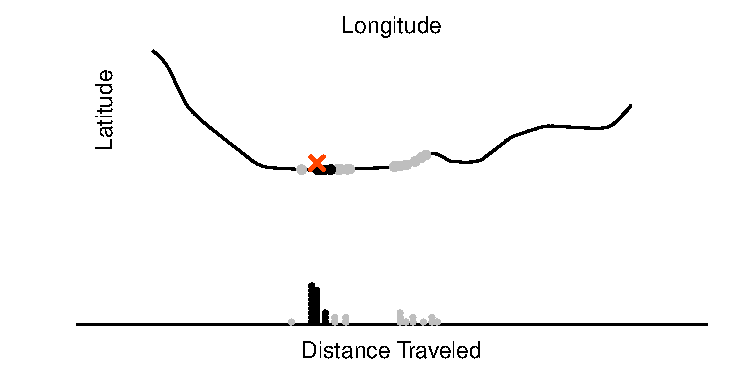
\includegraphics[width=\textwidth]{figures/03_particle_filter_4.pdf}
        \caption{Resampling occurs using likelihood weights that use the distance
            between the particle's location and the vehicles reported location (red cross),
            resulting in the updated state.}
        \label{fig:pf_state_predict2}
    \end{subfigure}
    \caption{The vehicles state is estimated using a set of discrete points, or particles,
        each of which is independently mutated to make predictions of the future state. The history of the state estimates can be used to estimate parameters of interest, such as
        travel times along roads.}
    \label{fig:pf_state}
\end{figure}




In a particle filter, the posterior distribution of the state at time $t_{k-1}$,
is represented by a set of discrete points, or particles, (fig~\ref{fig:pf_state_prev}),
each with an associated weight $W_{k-1}^{(i)}$
\begin{equation}
p(\bX_{k-1} | \bY_{k-1}) \approx \tilde\bX_{k-1|k-1} 
:= \{\bX_{k-1}^{(i)}, W_{k-1}^{(i)}\}_{i=1}^N
\end{equation}
each of which is independently updated or \emph{mutated} using the transition function $f$ (fig~\ref{fig:pf_state_predict})
\begin{equation}
p(\bX_k | \bX_{k-1}) \approx \tilde\bX_{k|k-1} := 
\left\{f(\bX_{k-1}^{(i)}, \psi), W_{k-1}^{(i)}\right\}_{i=1}^N
\end{equation}
using parameter vector $\psi$ containing all of the necessary parameters
for the model (including system noise).
After mutation, 
the particles are reweighted using the likelihood $p(\bY_k | \bX_k^{(i)})$ 
(sec.~\ref{sec:pf_update}) and standardised,
\begin{equation*}
W_k^{(i)} = \frac{W_{k-1}^{(i)} p(\bY_k | \bX_k^{(i)})}{
    \sum_{j=1}^N W_{k-1}^{(j)} p(\bY_k | \bX_k^{(j)})
}
\end{equation*}
generating a posterior estimate of the state
\begin{equation}
p(\bX_k | \bY_k) \approx \tilde\bX_{k|k} := 
\{\bX_{k}^{(i)}, W_{k}^{(i)}\}_{i=1}^N.
\end{equation}

In order to prevvent degeneration of the particle sample,
\emph{importance resampling} is employed whenever the 
effective sample size $N_{\text{eff}} = 1/(\sum_i (W_k^{(i)})^2)$
falls below a specified threshold $N_{\text{thres}}$.
The resampling is performed with replacement using importance weights $W_k^{(i)}$,
as demonstrated in Figure~\ref{fig:pf_state_update}.
Afterwards, the weights are reinitialized to $W_k^{(i)} = N^{-1}$.



\subsubsection{Vehicle transition function}
\label{sec:pf_prediction}

Using a particle filter allows us to develop a vehicle model in which
the transition function $f$ implements several key bus behaviours:
\begin{itemize}
\item non-constant speed along roads,
\item optional stopping and waiting at bus stops while passengers board and disembark, and
\item optional stopping and waiting at intersections/traffic lights (future work).
\end{itemize}

For each particle, the transition function generates a plausible trajectory,
using system noise parameter $\sigma^2$ which describes 
how the vehicle's acceleration changes as a random process.
The vehicle does not travel constantly along the route,
however, as it needs to service bus stops along the way.
Therefore, the transition function includes 
stopping probabilities $\boldsymbol\pi = (\pi_1,\ldots,\pi_J)^\top$ at bus stops,
dwell times $\boldsymbol\tau = (\tau_1,\ldots,\tau_J)^\top$ for passengers to
board and disembark (conditional on the bus stopping),
and the minimum dwell time at stops, $\gamma$,
for the doors to open and close.
For these parameters, we used constant values for all stops,
and based the values on those used by \cite{Hans_2015};
future work will investigate modeling these in real-time similarly to Section~\ref{sec:kf}.
No intersection model is implemented here,
as the segment road segments are between stops,
and the travel times predicted by the network model at time $t_k$,
$\btheta(t_k) = (\theta_1(t_k), \ldots, \theta_L(t_k))^\top$
(see section~\ref{sec:kf}).
The transition function algorithm is shown in Figure~\ref{fig:algorithm},
which implements those features discussed above.



\subsubsection{Updating state using the observation likelihood}
\label{sec:pf_update}

After mutating the particle set, the posterior distribution $\tilde\bX_{k|k}$ 
is updated by reweighting each particle using the likelihood.
The measurement function $h$,
and an additional function $g$ which transforms GPS coordinates onto a flat
surface (the geographical equirectangular projection),
allow the placement of a bivate normal likelihood on the data
as shown in figure~\ref{fig:pf_lhood}.
The model for the observation generation is,
assuming GPS error $\epsilon^2$,
\begin{equation}
\label{eq:pf_obs_model}
g(\bY_k) = g(h(\bX_k)) + \br_k,
\quad \br_k \sim \mathrm{N}(\boldsymbol{0}, \epsilon^2\boldsymbol{I})
\end{equation}
Now, the geographical distance between the observation and the true vehicle can be expressed
in terms of two independent random variables $z_1, z_2 \sim \mathrm{N}(0,1)$
\begin{equation}
\label{eq:obs_dist}
dist(\bY_k, h(\bX_k)) = \sqrt{r_{k1}^2 + r_{k2}^2} 
    = \sqrt{(\epsilon z_1)^2 + (\epsilon z_2)^2}.
\end{equation}
The sum of two independent, standard normal random variables 
is $\chi^2$ distributed with 2~degrees of freedom,
which is itself exponential,
so rearranging (\ref{eq:obs_dist}) yields
\begin{equation}
\label{eq:obs_exp}
\left(\frac{dist(\bY_k, h(\bX_k))}{\epsilon}\right)^2 =
z_1^2 + z_2^2 \sim \mathrm{Exp}\left(\frac{1}{2}\right)
\end{equation}

The likelihood of the data given a particle's state estimate 
is therefore easy to calculate using (\ref{eq:obs_exp})
\begin{equation}
p(\bY_k | \bX_k^{(i)}, \epsilon) =
\frac{1}{2}\exp\left\{
-\frac{1}{2} \left(\frac{dist(\bY_k, h(\bX_k^{(i)}))}{\epsilon}\right)^2
\right\}
\end{equation}
It is worth noting that this representation of the likelihood is only
possible due to the discretization of the state provided by the particle filter;
in other approaches, such as the Kalman filter,
the likelihood cannot be calculated using the distance as the estimate
is a distribution, and so instead a reverse non-deterministic transformation,
the inverse measurement function,
is required to estimate the ``observed'' distance traveled $\hat Z_k~=~h^{-1}(\bY_k)$, 
which introduces additional error and uncertainty into the model.



\subsection{Network model}
\label{sec:kf}

The purpose of the road network model is to provide a way of using
spatial information about vehicle speeds to inform arrival time predictions.
The simplest notion would be to map each vehicle speed estimate to a physical road;
however, this has two problems
\begin{enumerate}
\item roads usually have two directions, so vehicle directionality would need to be computed,
\item road data is not provided in GTFS, and can be difficult to obtain cleanly without
    manual intervention.
\end{enumerate}
The most desirable solution would be to use the GTFS shape data to construct a network
by merging overlapping routes and using merge points as intersections
to define road segments.
Initial efforts at applying this had poor results due to overly long or short segments,
so for this current work we are approximating the road network by using the stops 
along a route as intersection, and the legs between them as road segments,
as shown in Figure~\ref{fig:network_creation}.


To obtain reliable ETAs,
road travel times need to be estimated in \rt,
as this allows the model to react to congestion changes as detected by preceeding buses.
Future work will aim to construct a more complex model incorporating historical trends 
and correlations between roads, 
however for the current work we are demonstrating our approach
using a simple model,
in which each road segment is treated independently.

The model assums a Gaussian state distribution for travel time,
truncated necessarily at zero;
this will not be an issue as the state prediction and data will always be non-negative.
However, the model must be able to handle multiple observations in a single update,
which often occurs along major bus routes when several buses are traveling together.
Therefore we have chosen the information filter as our estimation method.

The information filter is a transormation of the Kalman filter in which the
\emph{information matrix} and \emph{information vector} are used in place of 
the covariance matrix and state vector, respectively.
The advantage is that multiple observations can be added together when updating the state.
Otherwise the information filter follows the same procedure as other recursive Bayesian models.

The network state $\boldsymbol\theta_c = \{\theta_c^\ell\}_{\ell = 1}^L$ is the travel time 
of transit vehicles along road segment $\ell$ at time $t_c$.
Observations of the state, $Z_c^\ell$, are obtained from the particle filter 
in Section~\ref{sec:pf}.
Due to the simplicity of the model,
no transition matrix or measurement matrix is required,
and the model from (\ref{eq:rbe_model}) reduces simply to
\begin{equation}
\begin{split}
\theta_c^\ell &= \theta_{c-1}^\ell + \Delta_c^\ell v_c^\ell \\
Z_c^\ell &= \theta_c^\ell + e_c^\ell
\end{split}
\end{equation}
where $\Delta_c = t_c - t_{c-1}$,
$v_c^\ell \sim \mathrm{N}(0, \nu^2)$ is the system noise,
and $e_c^\ell \sim \mathrm{N}(0, R_c^\ell)$ is the measurement error
as estimated from the vehicle model using uncertainty of particle estimates.

The state is estimated by its mean $\hat \theta_c^\ell = \mathrm{E}(\theta_c^\ell)$
and uncertainty $P_c^\ell = \mathrm{var}(\theta_c^\ell)$,
which are predicted from the previous state estimate using the prediction
equations
\begin{align*}
\label{eq:kf_transition}
\hat \theta^\ell_{c|c-1} &= \hat \theta^\ell_{c|c-1} \\
P^\ell_{c|c-1} &= P^\ell_{c-1|c-1} + \Delta_c^\ell \nu_c^\ell
\end{align*}

For the update step, the parameters are transformed into an information
space parameterised by the information matrix $U^\ell_c$
and the information vector $u^\ell_c$,
\begin{equation}
\label{eq:information_transform}
U^\ell_{c|c-1} = \frac{1}{P_{c|c-1}}
\quad\text{and}\quad
\hat u^\ell_{c|c-1} = \frac{\hat \theta^\ell_{c|c-1}}{P^\ell_{c|c-1}}
\end{equation}
The measurement data obtained from the vehicle model are
the travel time of vehicle $m$ along segment $\ell$,
$\bar z_c^{m\ell}$, and the uncertainty $s^{m\ell}_c$.
These are transformed to a measurement information covariance matrix $B_c^{m\ell}$
and measurement information vector $b_c^{m\ell}$,
\begin{equation*}
B^{m\ell}_c = \frac{1}{(s^{m\ell}_c)^{2}}\quad\text{and}\quad
b^{m\ell}_c = \frac{\bar z^{m\ell}_c}{(s^{m\ell}_c)^2}
\end{equation*}
The information update is now the sum of the information over all $M$ vehicles
that traversed the segment since the last update, so
\begin{align*}
U^\ell_{c|c} &= U^\ell_{c|c-1} + \sum_{m=1}^M B^{m\ell}_{c} \\
\hat u^\ell_{c|c} &= \hat u^\ell_{c|c-1} + \sum_{m=1}^M b^{m\ell}_{c}
\end{align*}
which are back transformed
using the inverse of (\ref{eq:information_transform})
to obtain the desired parameter estimates
\begin{equation*}
\hat \theta^\ell_{c|c} = \frac{\hat u^\ell_{c|c}}{U^\ell_{c|c}} 
\quad\text{and}\quad
P^\ell_{c|c} = \frac{1}{U^\ell_{c|c}}.
\end{equation*}



